\documentclass[hyperref]{beamer}
\usepackage{beamerthemesplit}
\usepackage{graphicx}
\usepackage{mathptmx}           % replacement for obsolete \usepackage{times}
\usepackage[scaled=1.0]{helvet} % replacement for obsolete \usepackage{times}
\usepackage{courier}            % replacement for obsolete \usepackage{times}
\usepackage[normalem]{ulem}

\usepackage{tikz}
\usetikzlibrary{shapes.arrows,chains,positioning,automata,trees,calc}
\usetikzlibrary{patterns}
\usetikzlibrary{decorations.pathmorphing,decorations.markings}
\usepackage{times,latexsym,amsfonts,amssymb,amsmath,graphicx,url,bbm,rotating,siunitx}
\usepackage{multirow,hhline,arydshln,array,color,stmaryrd,pifont}
\definecolor{darkred}{rgb}{0.5, 0.0, 0.0}
\definecolor{darkgreen}{rgb}{0.0, 0.4, 0.0}
\definecolor{darkblue}{rgb}{0.0, 0.0, 0.5}

% set up Beamer style with Stanford colors and logo
% logo is available at http://nlp.stanford.edu/local/nlp-logos/nlp-logo.pdf
\useinnertheme{rounded}
\useoutertheme{infolines}
\usecolortheme{beaver}
\setbeamercolor{block title}{fg=white,bg=darkred!75!black}
\setbeamercolor{block body}{parent=normal text,bg=black!5!bg}
\setbeamercolor{item projected}{bg=darkred}
\logo{
\includegraphics[height=1cm]{../../img/nlp-logo.pdf}}

% title page information
\title{NaturalLI: Natural Logic Inference for Common Sense Reasoning}
\subtitle{}
\author{Gabor Angeli, Chris Manning}
\date{October 42, 2014}
\institute[Stanford]{Stanford University}

\input ../../macros.tex
\input ../../figures.tex

\begin{document}
\begin{frame}
  \titlepage
\end{frame}

%%%%%%%%%%%%%%%%%%%%%%%%%%%%%%%%%%%%%%%%%%%%%%%%%%%%%%%%%%%%%%%%%%%%%%%%%%%%%%%%
%% MOTIVATION
%%%%%%%%%%%%%%%%%%%%%%%%%%%%%%%%%%%%%%%%%%%%%%%%%%%%%%%%%%%%%%%%%%%%%%%%%%%%%%%%
%
%%%%%%%%%%%%%%%%%%%% 
%% COMMON SENSE REASONING TEASER
%%%%%%%%%%%%%%%%%%%%
%\begin{frame}{\scalebox{0.95}{Natural Logic Inference for \uline{\textbf{Common Sense Reasoning}}}}
%\begin{tabular}{cc}
%  \green{Kittens play with yarn} & \red{Kittens play with computers} \\
%  \vspace{0.25cm} \\
%  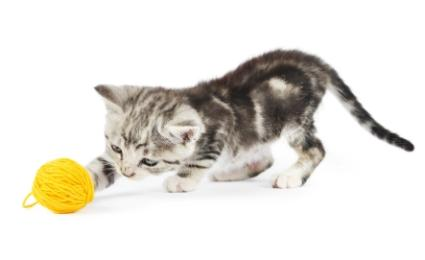
\includegraphics[width=5cm]{../../img/yarn-cat.jpg} & \pause 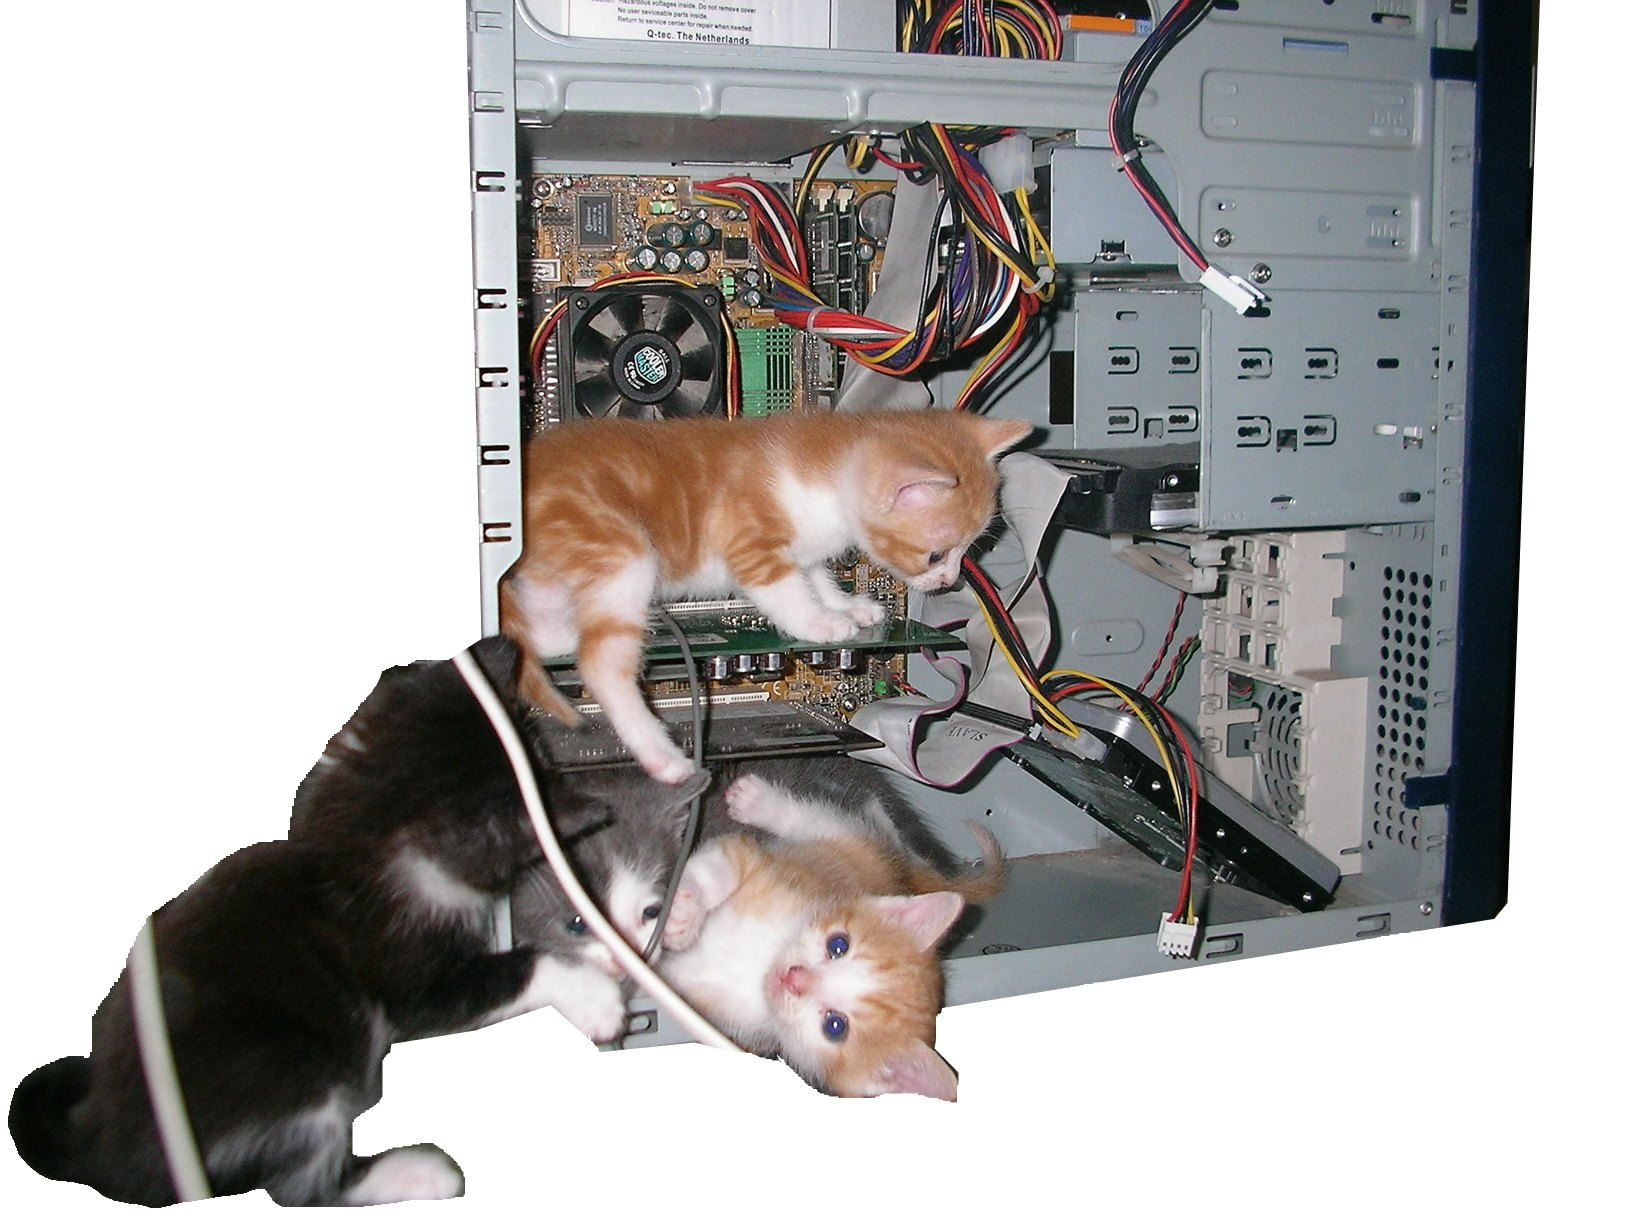
\includegraphics[width=5cm]{../../img/computer-cat-cropped.jpg}
%\end{tabular}
%\end{frame}
%
%%%%%%%%%%%%%%%%%%%% 
%% COMMON SENSE REASONING DEFN
%%%%%%%%%%%%%%%%%%%%
%\begin{frame}{\scalebox{0.95}{Natural Logic Inference for \uline{\textbf{Common Sense Reasoning}}}}
%\begin{center}
%\begin{tabular}{ll}
%  \hh{Input}  & A query fact (e.g., \w{cats have tails}). \\
%  & \\
%  \hh{Output} & \textbf{True} or \textbf{False}, with some confidence.
%\end{tabular}
%\end{center}
%\pause
%
%\vspace{0.5cm}
%\hh{Subtleties we ignore:}
%\begin{itemize}
%  \item \textbf{Truth is elusive.}
%    \begin{itemize}
%      \item \true{birds fly} but \false{penguins don't fly}.
%      \pause
%      \item \unknown{Obama is a good president}.
%      \pause
%      \item A fact is true if we would accept it without evidence to the contrary.
%    \end{itemize}
%  \pause
%  \item \textbf{The internet lies.}
%    \begin{itemize}
%      \item \false{Obama was born in Kenya}.
%    \end{itemize}
%  \pause
%  \item \textbf{This query is false.}
%\end{itemize}
%\end{frame}
%
%%%%%%%%%%%%%%%%%%%% 
%% COMMON SENSE REASONING NLP
%%%%%%%%%%%%%%%%%%%%
%\begin{frame}{\uline{\textbf{Common Sense Reasoning}} for NLP}
%\begin{center}
%  \w{The city refused the demonstrators a permit because they feared violence.} \\
%  \pause
%  \begin{tabular}{l}
%    \true{a city fears violence} \\
%    \false{demonstrators fear violence}
%  \end{tabular}
%\end{center}
%\pause
%
%\begin{center}
%  \w{I ate the cake with a cherry} \hspace{0.25cm} vs. \hspace{0.25cm} \w{I ate the cake with a fork} \\
%  \begin{tabular}{l}
%    \true{cakes come with cherries} \\
%    \false{cakes are eaten using cherries}
%  \end{tabular}
%\end{center}
%\pause
%
%\begin{center}
%  \w{Put a sarcastic comment in your talk. That's a great idea.} \\
%  \begin{tabular}{l}
%    \false{Sarcastic comments are a great idea in talks.}
%  \end{tabular}
%\end{center}
%
%\end{frame}
%
%%%%%%%%%%%%%%%%%%%% 
%% COMMON SENSE REASONING VISION
%%%%%%%%%%%%%%%%%%%%
%\begin{frame}{\uline{\textbf{Common Sense Reasoning}} for Vision}
%\begin{tabular}{cc}
%  \red{Dogs drive cars} & \green{People drive cars} \\
%  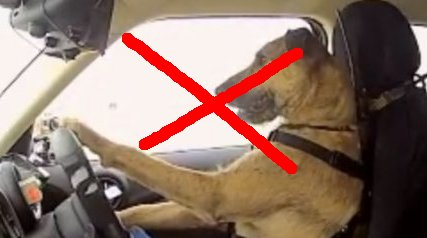
\includegraphics[height=3cm]{../../img/dog-driving.jpg} & 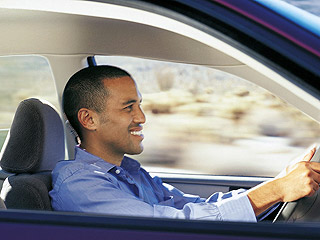
\includegraphics[height=3cm]{../../img/person-driving.jpg}  \\
%  \vspace{0.0cm} \\
%  \pause \red{Baseball is played underwater} & \green{Baseball is played on grass} \\
%  
\includegraphics[height=3cm]{../../img/baseball-underwater.jpg} & 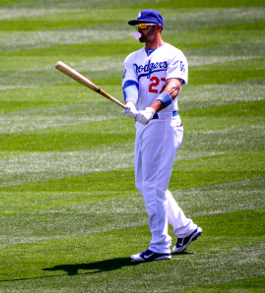
\includegraphics[height=3cm]{../../img/baseball-grass.jpg} \\
%\end{tabular}
%\end{frame}
%
%%%%%%%%%%%%%%%%%%%% 
%% TEASER
%%%%%%%%%%%%%%%%%%%%
%\begin{frame}{Start with a large knowledge base}
%\begin{center}
%  \teaserManyPremises
%\end{center}
%\end{frame}
%
%\begin{frame}[noframenumbering]{Infer new facts...}
%\begin{center}
%  \teaserBlindInferenceNaturalOrder
%\end{center}
%\end{frame}
%
%\begin{frame}[noframenumbering]{Infer new facts...on demand from a query...}
%\begin{center}
%  \teaserBlindInference
%\end{center}
%\end{frame}
%
%\begin{frame}[noframenumbering]{...Using text as the meaning representation...}
%\begin{center}
%  \teaserInference
%\end{center}
%\end{frame}
%
%\begin{frame}[noframenumbering]{...Without aligning to any particular premise.}
%\begin{center}
%  \teaserFullDerivation
%\end{center}
%\end{frame}
%
%
%%%%%%%%%%%%%%%%%%%% 
%% INFERENCE MOTIVATION
%%%%%%%%%%%%%%%%%%%%
%\begin{frame}{\scalebox{0.95}{Natural Logic \uline{\textbf{Inference}} for Common Sense Reasoning}}
%\begin{center}
%  \teaserBlindInferenceNaturalOrder
%\end{center}
%\end{frame}
%
%\begin{frame}[noframenumbering]{\scalebox{0.95}{Natural Logic \uline{\textbf{Inference}} for Common Sense Reasoning}}
%\hh{Lots of common sense knowledge bases:}
%\begin{itemize}
%  \item OpenIE (TextRunner, ReVerb, Ollie, OpenIE4).
%  \item NELL, ConceptNet (OpenMind Common Sense), OpenCyc, etc.
%\end{itemize}
%\vspace{0.5cm}
%\pause
%
%\hh{A key challenge is coverage.}
%\pause
%\begin{itemize}
%  \item We can greatly improve coverage with \textit{inference}.
%\end{itemize}
%\vspace{0.5cm}
%\pause
%
%\hh{Contrast: RTE challenges.}
%\begin{itemize}
%  \item \red{Few premises}; \green{many inference steps}.
%\end{itemize}
%\pause
%
%\hh{Contrast: Relation inference.}
%\begin{itemize}
%  \item \green{Many premises}; \red{few inference steps}.
%\end{itemize}
%\end{frame}
%
%\begin{frame}[noframenumbering]{\scalebox{0.95}{Natural Logic \uline{\textbf{Inference}} for Common Sense Reasoning}}
%\begin{center}
%  \teaserBlindInferenceNaturalOrder
%\end{center}
%\end{frame}
%\begin{frame}[noframenumbering]{\scalebox{0.95}{Natural Logic \uline{\textbf{Inference}} for Common Sense Reasoning}}
%\begin{center}
%  \teaserBlindInference
%\end{center}
%\end{frame}
%
%%%%%%%%%%%%%%%%%%%% 
%% NATLOG MOTIVATION
%%%%%%%%%%%%%%%%%%%%
%\begin{frame}{Properties of an inference algorithm}
%\hh{Want to make many inference steps}
%\begin{itemize}
%  \item[$\Rightarrow$] Computationally fast during inference.
%\end{itemize}
%\pause
%\vspace{0.5cm}
%
%\hh{Want to leverage large knowledge base}
%\begin{itemize}
%  \item[$\Rightarrow$] Computationally fast during pre-processing.
%\end{itemize}
%\pause
%\vspace{0.5cm}
%
%\hh{Still want to capture common inferences}
%\pause
%\vspace{0.5cm}
%
%\begin{center}
%  \begin{tabular}{rl}
%    \multicolumn{1}{m{3cm}}{
\includegraphics[width=3cm]{../../img/superhero.pdf}} &
%    \huge{Natural Logic}
%  \end{tabular}
%\end{center}
%\end{frame}
%
%
%%%%%%%%%%%%%%%%%%%%%%%%%%%%%%%%%%%%%%%%%%%%%%%%%%%%%%%%%%%%%%%%%%%%%%%%%%%%%%%%
%% NATURAL LOGIC
%%%%%%%%%%%%%%%%%%%%%%%%%%%%%%%%%%%%%%%%%%%%%%%%%%%%%%%%%%%%%%%%%%%%%%%%%%%%%%%%
%
%%%%%%%%%%%%%%%%%%%% 
%% NATLOG AS SYLLOGISMS
%%%%%%%%%%%%%%%%%%%%
%\begin{frame}{\scalebox{0.95}{\uline{\textbf{Natural Logic}} Inference for Common Sense Reasoning}}
%\begin{center}
%  \teaserInference
%\end{center}
%\end{frame}
%
%\begin{frame}[noframenumbering]{Natural Logic as Syllogisms}
%\begin{center}
%  \hh{s/Natural Logic/Syllogistic Reasoning/g}
%\end{center}
%\vspace{0.25cm}
%\pause
%
%\hh{Quantifiers are important}
%\vspace{0.25cm}
%\hspace{0.5cm}
%\begin{tabular}{lp{4cm}lp{5cm}}
%  &\textbf{All} Greeks are mortal & & \textbf{Some} Greeks are women \\
%  &Socrates is Greek & & Socrates is Greek \\
%  $\therefore$& \true{Socrates is Mortal} & $\therefore$ & \false{Socrates is a woman} \\
%\end{tabular}
%\vspace{0.5cm}
%\pause
%
%\hh{Half the premises are in WordNet} \\
%\vspace{0.25cm}
%\hspace{0.5cm}
%\begin{tabular}{lp{6cm}}
%  &\textbf{Some} cat ate a mouse \\
%  &\sout{Cats are carnivores} \\
%  &\sout{Mice are animals} \\
%  $\therefore$& \true{Some carnivore ate an animal} \\
%\end{tabular}
%\vspace{0.5cm}
%\pause
%
%\hh{Logic of \textit{lexical mutations} warranted by governing quantifiers.}
%\end{frame}
%
%%%%%%%%%%%%%%%%%%%% 
%% NATLOG ANIMATION
%%%%%%%%%%%%%%%%%%%%
%\input example.tex
%
%%%%%%%%%%%%%%%%%%%% 
%% BEYOND SYLLOGISMS
%%%%%%%%%%%%%%%%%%%%
%\input extensions.tex
%
%%%%%%%%%%%%%%%%%%%% 
%% ADVANTAGES OF NATLOG
%%%%%%%%%%%%%%%%%%%%
%\begin{frame}{Properties of Natural Logic}
%\begin{itemize}
%  \item[\green{\checkmark}] Computationally fast during inference.
%  \begin{itemize}
%    \item ``Semantic'' parse of query is just syntactic parse.
%    \item Inference is lexical mutations / insertions / deletions.
%  \end{itemize}
%  \vspace{0.5cm}
%  \pause
%
%  \item[\green{\checkmark}] Computationally fast during pre-processing.
%  \begin{itemize}
%    \item Plain text!$^*$
%    \pause
%    \item[] ($^*$Generated from Ollie extractions.)
%  \end{itemize}
%  \vspace{0.5cm}
%  \pause
%
%  \item[\green{\checkmark}] Still captures common inferences.
%  \begin{itemize}
%    \item We make these types of inferences regularly and instantly.
%    \pause
%    \item We expect \textit{readers} to make these inferences instantly.
%  \end{itemize}
%\end{itemize}
%\end{frame}
%
%%%%%%%%%%%%%%%%%%%%%%%%%%%%%%%%%%%%%%%%%%%%%%%%%%%%%%%%%%%%%%%%%%%%%%%%%%%%%%%%
%% INFERENCE
%%%%%%%%%%%%%%%%%%%%%%%%%%%%%%%%%%%%%%%%%%%%%%%%%%%%%%%%%%%%%%%%%%%%%%%%%%%%%%%%
%
%%%%%%%%%%%%%%%%%%%% 
%% INFERENCE IS SEARCH
%%%%%%%%%%%%%%%%%%%%
%\begin{frame}{Natural Logic Inference is Search}
%  \teaserFullDerivation
%\end{frame}
%
%\begin{frame}[noframenumbering]{Natural Logic Inference is Search}
%\begin{center}
%  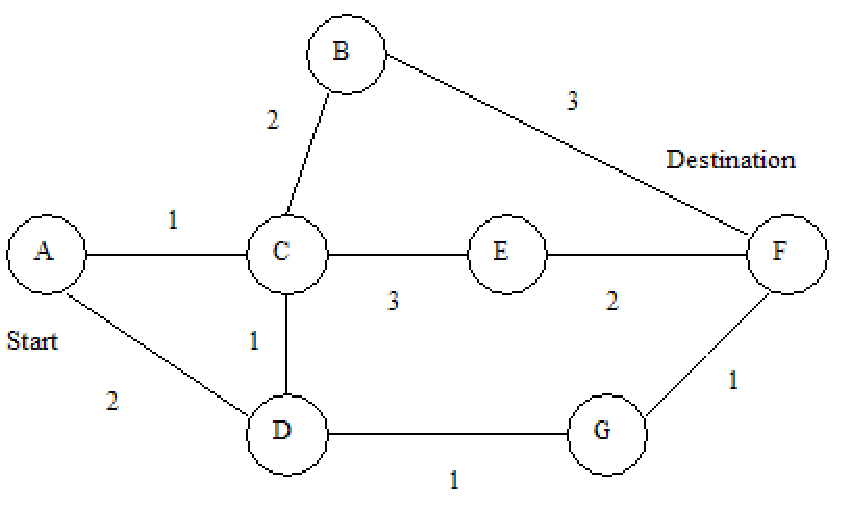
\includegraphics[width=5cm]{../../img/dijkstras-graph.pdf}
%\end{center}
%\begin{tabular}{ll}
%  \hh{Nodes} & $($ \w{fact}, validity $\in\{\textrm{valid}, \textrm{invalid}\})$ \\
%  & \\
%  \pause
%  \hh{Start Node} & \w{query fact} \\
%  \hh{End Nodes}  & \w{any known fact} \\
%  & \\
%  \pause
%  \hh{Edges} & Mutations of the current fact \\
%  \pause
%  \hh{Edge Costs} & How ``wrong'' an inference step is (learned). \\
%\end{tabular}
%\end{frame}
%
%%%%%%%%%%%%%%%%%%% 
%% EXAMPLE SEARCH
%%%%%%%%%%%%%%%%%%%
%\input exampleSearch.tex
%
%%%%%%%%%%%%%%%%%%%% 
%% EDGE TEMPLATES
%%%%%%%%%%%%%%%%%%%%
%\begin{frame}{Edge Templates}
%\begin{center}
%  \begin{tabular}{p{0.4\textwidth}p{0.20\textwidth}}
%    \multicolumn{1}{c}{\textbf{Template}} & \multicolumn{1}{c}{\textbf{Instance}} \\
%    & \\
%    Hypernym & \w{animal} $\rightarrow$ \w{cat} \\
%    Hyponym  & \w{cat} $\rightarrow$ \w{animal} \\
%    Antonym  & \w{good} $\rightarrow$ \w{bad} \\
%    Synonym  & \w{cat} $\rightarrow$ \w{true cat} \\
%    Add Word  & \w{cat} $\rightarrow$ \w{$\cdot$} \\
%    Delete Word  & $\cdot$ $\rightarrow$ \w{cat} \\
%    Quantifier Weaken & \w{some} $\rightarrow$ \w{all} \\
%    Quantifier Strengthen & \w{all} $\rightarrow$ \w{some} \\
%    Quantifier Negate & \w{all} $\rightarrow$ \w{no} \\
%    Quantifier Synonym & \w{all} $\rightarrow$ \w{every} \\
%    \pause \\
%    Nearest Neighbor  & \w{cat} $\rightarrow$ \w{dog} \\
%  \end{tabular}
%\end{center}
%\end{frame}
%
%
%%%%%%%%%%%%%%%%%%%% 
%% DELETIONS (INSERTIONS)
%%%%%%%%%%%%%%%%%%%%
%\begin{frame}{Inserting Words During Search}
%\begin{center}
%  \scalebox{0.8}{\wordthe \cat \eat \mice}
%\end{center}
%\end{frame}
%
%\begin{frame}[noframenumbering]{Inserting Words During Search}
%\begin{center}
%  \scalebox{0.8}{\wordthe \cat \eat \worda \mice}
%\end{center}
%\end{frame}
%
%\def\worda{\monoUpR{}{???}{}{}}
%\begin{frame}[noframenumbering]{Inserting Words During Search}
%\begin{center}
%  \scalebox{0.8}{\wordthe \cat \eat \worda \mice} \\
%  \vspace{0.5cm}
%  \exampleInsertions
%\end{center}
%\end{frame}
%
%%%%%%%%%%%%%%%%%%%% 
%% STORE FACTS AS A TRIE
%%%%%%%%%%%%%%%%%%%%
%\def\title{Store Facts as a Trie}
%\begin{frame}{\title}
%  \factTrie{dotpath}{dotpath}{dotpath}
%\end{frame}
%
%\begin{frame}[noframenumbering]{\title}
%  \factTrie{goodPath}{dotpath}{dotpath}
%\end{frame}
%
%\begin{frame}[noframenumbering]{Inserting Words During Search}
%\begin{center}
%  \scalebox{0.8}{\wordthe \cat \eat \worda \mice}
%\end{center}
%\end{frame}
%
%\def\worda{\monoUpR{}{catnip}{herb}{tracheophyte}}
%\begin{frame}[noframenumbering]{Inserting Words During Search}
%\begin{center}
%  \scalebox{0.8}{\wordthe \cat \eat \worda \mice}
%\end{center}
%\end{frame}
%
%\begin{frame}[noframenumbering]{\title}
%  \factTrie{dotpath}{goodPath}{dotpath}
%\end{frame}
%
%\def\worda{\monoUpR{}{???}{}{}}
%\begin{frame}[noframenumbering]{Inserting Words During Search}
%\begin{center}
%  \scalebox{0.8}{\wordthe \cat \eat \worda \mice}
%\end{center}
%\end{frame}
%
%\def\worda{\monoUpR{}{my}{}{}}
%\begin{frame}[noframenumbering]{Inserting Words During Search}
%\begin{center}
%  \scalebox{0.8}{\wordthe \cat \eat \worda \mice}
%\end{center}
%\end{frame}
%
%\begin{frame}[noframenumbering]{\title}
%  \factTrie{dotpath}{dotpath}{goodPath}
%\end{frame}
%
%\def\worda{\monoUpR{}{???}{}{}}
%\begin{frame}[noframenumbering]{Inserting Words During Search}
%\begin{center}
%  \scalebox{0.8}{\wordthe \cat \eat \worda \mice}
%\end{center}
%\end{frame}
%
%\def\worda{\monoUpR{\textbf{All$_{\downarrow \uparrow}$}}{\darkgreen{\textbf{a$_{\uparrow \uparrow}$}}}{}{}}
%\begin{frame}[noframenumbering]{Inserting Words During Search}
%\begin{center}
%  \scalebox{0.8}{\wordthe \cat \eat \worda \mice}
%\end{center}
%\end{frame}

%%%%%%%%%%%%%%%%%%% 
% CONTRIBUTION: COLLAPSED INFERENCE STATES
%%%%%%%%%%%%%%%%%%%
\def\title{Contribution: The Missing Slides}
\def\blurb{
\hh{Inference according to us:} The truth of a node is \textit{maintained} or
  \textit{flipped} based on the template of the outgoing edge}
\begin{frame}{\title}
\blurb.
\end{frame}

\begin{frame}[noframenumbering]{\title}
\blurb\ \darkgreen{\textbf{and the truth of the node}}.
\end{frame}

\begin{frame}[noframenumbering]{\title}
\blurb\ and the truth of the node 
  \darkgreen{\textbf{and the exact quantifiers in scope}}.
\end{frame}

\def\blurb{
\hh{Inference according to us:} The truth of a node is \textbf{\textit{maintained} or
  \textit{flipped}} based on the template of the outgoing edge and the truth of the node 
  and the exact quantifiers in scope.
}
\begin{frame}[noframenumbering]{\title}
\blurb
\end{frame}


\def\joinTable{
  \begin{tabular}{|c||c|c|c|c|c|c|c|}
    \hline
    $\bowtie$ & $\equivalent$ & $\forward$ & $\reverse$ & $\negate$ & $\alternate$ & $\cover$ & $\independent$ \\
    \hline
    $\equivalent$ & $\equivalent$ & $\forward$ & $\reverse$ & $\negate$ & $\alternate$ & $\cover$ & $\independent$ \\
    $\forward$ & $\forward$ & $\forward$ & $\independent$ & $\alternate$ & $\alternate$ & $\independent$ & $\independent$ \\
    $\reverse$ & $\reverse$ & $\independent$ & $\reverse$ & $\cover$ & $\independent$ & $\cover$ & $\independent$  \\
    $\negate$ & $\negate$ & $\cover$ & $\alternate$ & $\equivalent$ & $\reverse$ & $\forward$ & $\independent$  \\
    $\alternate$ & $\alternate$ & $\independent$ & $\alternate$ & $\forward$ & $\independent$ & $\forward$ & $\independent$  \\
    $\cover$ & $\cover$ & $\cover$ & $\independent$ & $\reverse$ & $\reverse$ & $\independent$ & $\independent$  \\
    $\independent$ & $\independent$ & $\independent$ & $\independent$ & $\independent$ & $\independent$ & $\independent$ & $\independent$ \\
    \hline
	\end{tabular}
}
\begin{frame}[noframenumbering]{\title}
\blurb \\
\begin{center}	
  \w{mammal} \reverse\ \w{cat} $~~\vdash~~$ \w{all mammals have fur} $\forward$ \w{all cats have fur} \\
  \pause
  \vspace{0.25cm}
  \joinTable
\end{center}
\end{frame}

\begin{frame}[noframenumbering]{\title}
\blurb \\
\begin{center}	
  \uline{\w{mammal} \reverse\ \w{cat}} $~~\vdash~~$ \w{all mammals have fur} $\forward$ \w{all cats have fur} \\
  \vspace{0.25cm}
  \joinTable
\end{center}
\end{frame}

\begin{frame}[noframenumbering]{\title}
\blurb \\
\begin{center}	
  \w{mammal} \reverse\ \w{cat} $~~\vdash~~$ \uline{\w{all mammals have fur} $\forward$ \w{all cats have fur}} \\
  \vspace{0.25cm}
  \joinTable
\end{center}
\end{frame}

\begin{frame}[noframenumbering]{\title}
\blurb \\
\begin{center}	
  \w{mammal} \reverse\ \w{cat} $~~\vdash~~$ \uline{\w{all mammals have fur} $\Rightarrow$ \w{all cats have fur}} \\
  \vspace{0.25cm}
  \joinTable
\end{center}
\end{frame}

%%%%%%%%%%%%%%%%%%%%%%%%%%%%%%%%%%%%%%%%%%%%%%%%%%%%%%%%%%%%%%%%%%%%%%%%%%%%%%%
% LEARNING
%%%%%%%%%%%%%%%%%%%%%%%%%%%%%%%%%%%%%%%%%%%%%%%%%%%%%%%%%%%%%%%%%%%%%%%%%%%%%%%

%%%%%%%%%%%%%%%%%%%%%%%%%%%%%%%%%%%%%%%%%%%%%%%%%%%%%%%%%%%%%%%%%%%%%%%%%%%%%%%
% RESULTS
%%%%%%%%%%%%%%%%%%%%%%%%%%%%%%%%%%%%%%%%%%%%%%%%%%%%%%%%%%%%%%%%%%%%%%%%%%%%%%%

\end{document}
